\documentclass[a4paper]{article}
\usepackage{geometry}
\usepackage{amsmath}
\usepackage{multicol}
\usepackage{graphicx}
\geometry{margin=0.25in}
\newcommand{\hrl}{
    \vspace{2mm}
    \hrule
    \vspace{2mm}
}

\setlength{\parindent}{0pt}


\begin{document}
\begin{multicols}{3}
\setlength{\abovedisplayskip}{2pt}
\setlength{\belowdisplayskip}{0pt}
Chapter 6 - BJTs
You need to go to page 357 in the text and find a bunch of the good
expressions relating $I_E$, $I_B$ and $I_C$.

$I_S$ is known as Saturation Current

We need to consider:\\
Base current $I_B$\\
Collector current $I_C$ and \\
Collector-emitter Voltage $V_{CE}$

$$i_C=I_s e^{v_{BE}/V_T}$$

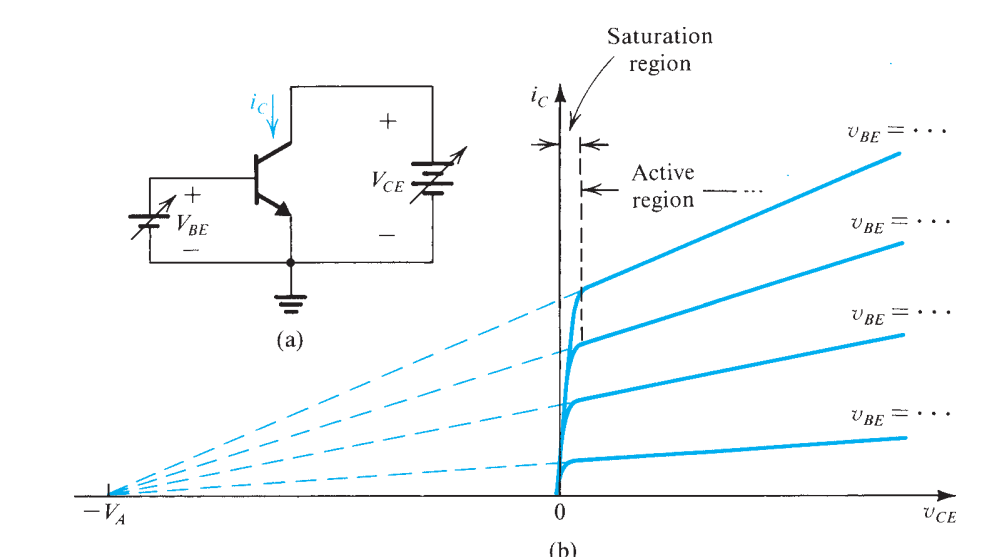
\includegraphics[width=\linewidth]{imgs/slopes.png}

Considering the Early voltage

$$i_C=I_s e^{v_{BE}/V_T} \left(1 + \frac{v_{CE}}{V_A}\right)$$
$$r_o=\left[\frac{\delta i_c}{\delta v_{CE}}\Big|_{V_{BE} = \text{constant}}\right]^{-1}$$
$$r_o=\frac{V_A + V_{CE}}{I_C}$$
$$r_o=\frac{V_A}{I_C^{'}}$$
Where $I_C^{'}=I_s e^{V_{BE}/V_T}$

\hrl
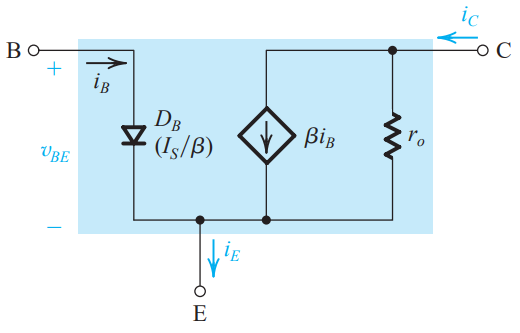
\includegraphics[width=\linewidth]{imgs/bjt_model.png}

$$ R_{CE_\text{SAT}} \equiv \frac{\delta v_{CE}}{\delta i_C} \Big|_{i_B = I_B \mid i_C=I_{C_\text{SAT}}}$$
$$ \frac{I_C}{I_B} = \text{transistor}~\beta $$



\end{multicols}

\end{document}